\documentclass[a4paper, oneside]{memoir}% Document class
\usepackage[a4paper]{geometry}			% Margins
\usepackage{lmodern}
\usepackage{graphicx}
\usepackage{float}
\usepackage{listings}
\usepackage[small,compact]{titlesec}	% No 'chapter' in chapter headings.
\graphicspath{{Media/}}					% Directory that holds images.

\titleformat{\chapter}[hang]
{\normalfont\Large\bfseries}{\thechapter}{1em}{\Large}
\titlespacing{\chapter}{0pt}{*0}{*1}

\titleformat{\chapter}{\Huge\bfseries}{\thechapter}{1em}{}
\titleformat{\section}{\LARGE\bfseries}{\thesection}{1em}{}
\titleformat{\subsection}{\Large\bfseries}{\thesubsection}{1em}{}
\titleformat{\subsubsection}{\normalsize\bfseries}{\thesubsubsection}{1em}{}


\author{
  Erik Sidelmann Jensen\\
  \texttt{ejens11@student.aau.dk}
  \and
  Lasse Vang Gravesen\\
  \texttt{lgrave11@student.aau.dk}
  \and
  Dennis Jakobsen\\
  \texttt{djakob11@student.aau.dk}  
}

\title{Web Intelligence - Social Media Miniproject}
\date{}

\begin{document}
	\clearpage\maketitle
	\thispagestyle{empty}
	
	\chapter{Social Media Miniproject}
	\section{Network Communities Partitioning}
	Community partitioning was done using spectral clustering.
	
	The general algorithm behind spectral clustering is this:
	\begin{enumerate}
	\item Given an adjacency matrix, A, representing a graph and an diagonal matrix D where the diagonal entry $i$ is the sum of $i$'th row in A. Compute the unnormalized Laplacian $L$ using $L = D-A$.
	\item Compute the second eigenvector $v_2$ of $L$, the one with the second smallest eigenvalue - not 0.
	\item The j'th value in the eigenvector corresponds to the j'th node.
	\item Order the nodes according to their eigenvector values.
	\item Cut at the largest gap.
	\end{enumerate}
	
	An example of this can be seen in the figure below.
	
	\begin{figure}[H]
	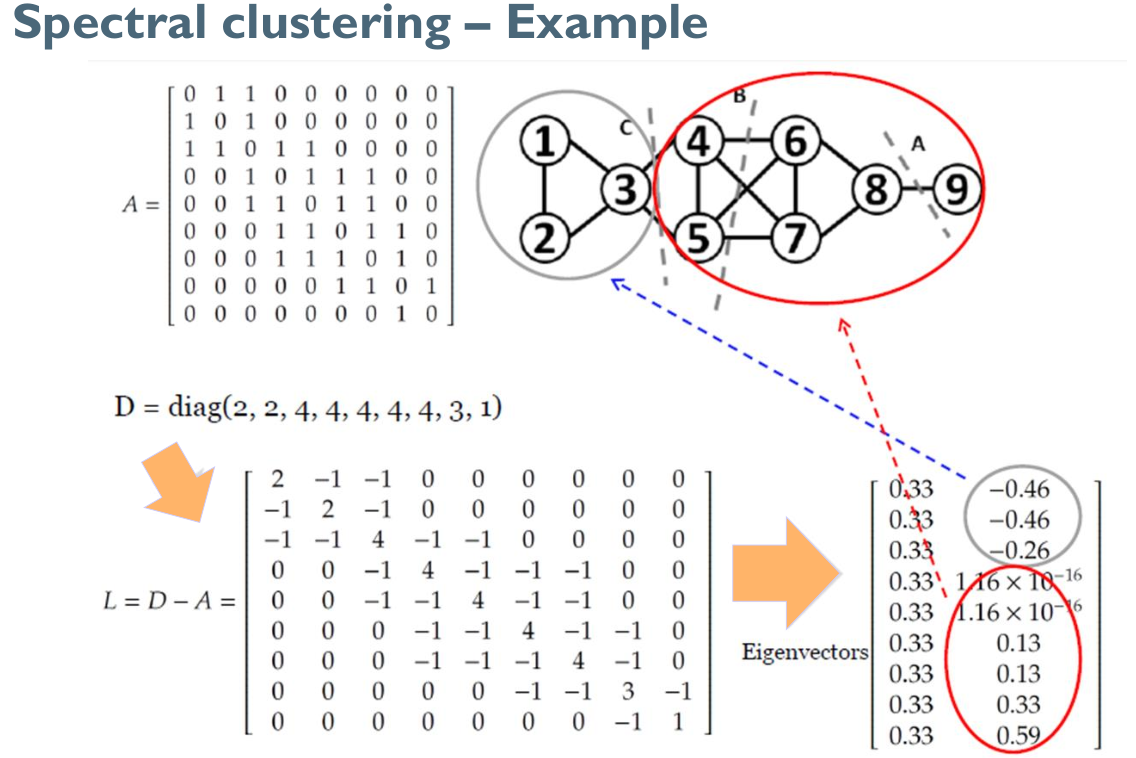
\includegraphics[scale=0.33]{SpectralClustering.png}
	\end{figure}
	
	To do this in practice the following was done:
	
	A User class was created to hold the basic information, the Username, the list of friends, the review, the summary, and a sortable eigen value. 
	Using this as a model the file containing the friendships and reviews could be loaded into a list of User objects.
	From this list of Users, the adjacency matrix A is created based on who they are friends with.
	From A, D is created
	The laplacian is calculated using L = D - A. 
	The eigen decomposition is then found on L, and the second smallest eigenvector is found. This is the computation of the second vector.
	The corresponding eigenvector-value is then assigned to a User object in the user list, after which the user list can be sorted.
	Then the largest gap can be cut. 
	
	To find more communities, this is then run recursively until a threshold gap of 0.7 is reached after which it stops and returns the list of communities. Alternatively to running it recursively, multiple eigenvectors could have been used to perform the cut. Also alternatively to the threshold gap, modularity could have been used.
	
	The results of this is 4 very segregated communities, on the first run-through the communities are obvious as can be seen in the figure below.
	
	\begin{figure}[H]
	
\includegraphics[scale=0.15]{matrix.png}
	\end{figure}
	
	The spectral clustering algorithm was used because it is simple to implement, and works well.
	
	\section{Sentiment Analysis}
	Sentiment analysis of text was done using a Naive Bayes Classifier.
	
	This was the procedure:
	First step is tokenising the test data and constructing features, and for sentiment analysis it is important to remember things like emoticons and negative words because those have an impact on the rest of the content. As such we took a sentiment sensitive tokeniser made in Python and converted it to C\#, and added sensitivity to negative words, in that every token followed by a negative word would get "\_NEG" appended until the end of the sentence(punctuation or an emoticon).
	
	The second step was parsing the learning data, which was done line by line, skipping the identifying text and taking the rest after having trimmed the result. Tokenising is also done in the parser, the tokeniser is called and these tokens are saved in a properties. Finally the known score of the review block is determined by the score. If the score is 3, the review is discarded. These reviews are then split into N partitions for easy learning and testing.
	
	The third step is then constructing the Naive Bayes Classifier, which is essentially just counting. Specifically these properties of the learning data is determined through counting:
	
	Estimation of the probability for all classes: $p(c)$. This is done through counting the amount of reviews available: N. The number of reviews with sentiment $c$: $N(c)$. We also have $|C|$, the amount of classes. Finally $p(c)$ can be estimated through
	
	$$p(c) = \frac{N(c) + 1}{N +|C|}$$
	
	We also estimate probability for all words in corpus $X$ and all possible sentiment classes in C: $p(x_i | c)$. 
	To do this we need to count the number of times $x_i$ appears across all reviews with sentiment c: $N(x_i, c)$. We also need $|X|$, the size of the vocabulary. Using this we can then calculate $p(x_i|c)$:
	
	$$(x_i|c) = \frac{N(x_{i}, c) + 1}{N(c) + |X|}$$
	
	Then the score for a review can be determined through two tricks:
	First calculate score for the "empty" review because most words from the vocabulary are not present in a given review(Trick 1). This is done using summation instead of product to avoid numerical instability(Trick 2).
	
	$$s^{*}(empty, c) = (\sum\limits_{i=1}^{n} p(\text{not } x_i | c)) + p(c)$$
	
	The score can then be calculated using:
	
	$$s(x, c) = s^{*}(empty, c) + (\sum\limits_{j=1}^{k} \frac{p(x_{j}|c)}{p(\text{not } x_{j}|c)})$$
	
	And that is how the Naive Bayes Classifier works, you first use the learning data to construct the probabilities and then you use those probabilities to determine the score for individual reviews.
	
	To test the classifier we used all possible combinations of test and learning data, where test data was 1 partition and learning data was the rest. So over N partitions, that means we iteratively ran over the partitions, selected the first for testdata, the rest for learning data and then in the second iteration we select the second for testdata and so on.
	
	Using this to improve the feature construction, we ended up with an accuracy rate of roughly 91\% and an error rate of roughly 9\% for each iteration. Though the classifier ended up being biased towards positive reviews in that it correctly classified them roughly 94\% of the time, and for negative reviews it classified them correctly roughly 77\% of the time.
	
	Alternatively to the Naive Bayes Classifier, MaxEnt could have been used and would probably have been a good choice since it apparently gives better results than Naive Bayes. It is more complicated however, and Naive Bayes works fine for our purposes. 
	
	\section{Evaluation of Reviews}
	We then used the community partitions and the sentiment classifier to evaluate the reviews. 

	We did this by using the entirety of the learning data to teach the Naive Bayes Classifier.
	We then ran through the list of users and classified the reviews of users that had reviews/summaries using the Naive Bayes Classifier.
	Then we determine the communities using the spectral clustering.
	Then we ran through the list of users again, this time only focusing on the users that did not have any reviews or summaries, and based on their friends average review scores we determine if they are likely to purchase. A user named 'kyle' and friends in other communities count 10 times more than a regular friend, finally we determine if they are likely to purchase by checking if the average is more than or equal to 3, and if it is the user is likely to purchase otherwise not.
	
	Our result in summary is then as follows:
	We classified 1347 user reviews out of 1644 as 'Positive', and 297 user reviews as 'Negative'.
	Of the users that did not have a review or a summary, we classified 2451 out of 2575 as likely to purchase and 124 as unlikely to purchase.	

\end{document}
